\section{Organisation du projet}
\label{sec:organisation}
    Le projet s’organise en deux phases distinctes. La phase d’analyse et de conception, qui consiste à analyser
    les besoins et les objectifs du projet (ce afin de faire un choix sur les technologies
    nécessaires à la réalisation de l’application), au découpage des tâches principales
    qui seront réalisées par la suite, et la réalisation de l’architecture principale avec
    la base de données envisagée. On sera amené
    à effectuer des tests pour voir ce qu’il est possible de faire avec la technologie envisagée,
    et on réalisera aussi une ébauche qui permettra d’avancer plus rapidement par la suite.

    Cette phase donnera lieu à 3 rapports. Ce rapport de pré-étude décrivant le contexte du projet,
    l’étude de l’art et une analyse des solutions possibles. Nous rédifgerons ensuite un  rapport de spécifications fonctionnelles
    qui détaillera la solution envisagée, les fonctionnalités détaillées de la plateforme et l’architecture
    de celle-ci, puis enfin le document de planification initial qui détaillera le calendrier des tâches
    et l’ordonnancement de celles-ci. Deux soutenances auront lieu suite à cette phase ; la première pour
    présenter le projet et la seconde pour présenter la planification initiale du développement de la plateforme.

    Pour cette phase chacun des membres du projet s’est retrouvé à chercher et étudier des sites proposant
    des services similaires à la plateforme que nous allons réaliser, ce afin de voir ce qui se fait aujourd’hui
    pour obtenir des idées sur les fonctionnalités à proposer essentielles pour ne pas faire moins bien
    que la concurrence, mais aussi récupérer des idées sur des options que nous aurions pu ne pas penser.
    Puis par la suite certains ont effectué des recherches sur les technologies que nous pourrions utiliser
    pour réaliser cette application. Par la suite, dans le cadre de la réalisation du document des spécifications
    fonctionnelles, seul ou par groupe chaque personne réalisera un ‘proof of concept’ avec les technologies trouvées
    pour voir ce que l’on peut faire, mais aussi pour comparer les résultats, faire un choix de technologie,
    et détailler toutes les tâches de conception en détail. Un travail de modélisation et d’ébauche sera partagé
    dans le groupe afin de pouvoir démarrer efficacement la phase de conception.

    La phase de conception, réalisée au second semestre avec Marlène, Romain et Alexandre, consistera au développement
    même de l’application, dont l’ébauche aura été réalisée durant la première phase. Le développement de l’application
    se fera avec le gestionnaire de version Git,  sur le Gitlab fourni par l’INSA.

    \pagebreak

    \subsection{Planning de la phase d’analyse}
    \label{subsec:planing}

    \begin{figure}[H]
        \centering
        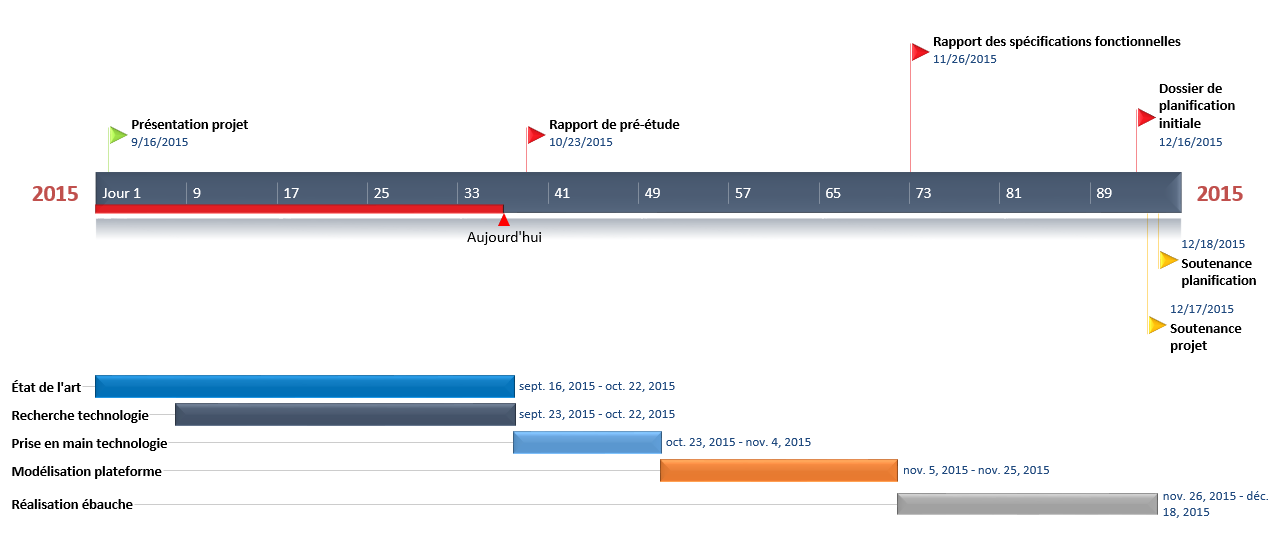
\includegraphics[width=1.3\textwidth, angle=90]{figure/timeline.png}
            \caption{Liste descriptive des tâches du planning d'analyse}
            \label{fig:description}
    \end{figure}

\section{Conclusion}
\label{Conclusion}
La numérisation de documents anciens est une problématique récente qui commence à toucher de plus en plus de monde.
Que ce soit par soucis de praticité ou de partage d’informations, on constate de plus en plus de sites archivant
de nombreux documents anciens, proposant plus ou moins de fonctionnalités. Certains sites sont d’ailleurs
consacrés spécifiquement à la presse ancienne, mais ceux-ci concernent les journaux provenant d’un pays
et sont plus ou moins accessibles, certains étant payants.

Plusieurs plateformes proposant des services similaires à ce que nous souhaitons proposer, un des challenges
de ce projet sera de pouvoir proposer toutes les fonctionnalités essentielles pour cette plateforme, et ce
tout en offrant un service unique qui nous permettrait de nous démarquer des autres services.

Ainsi nous souhaitons proposer aux utilisateurs une plateforme permettant de trouver efficacement et rapidement
tout journal présent dans notre base de données, une navigation fluide et complète dans chaque journal permettant
de situer et trouver facilement des articles, des images ou du texte dans les pages de journaux qui peuvent
atteindre de très grandes tailles. Enfin proposer un espace collaboratif, où les utilisateurs pour créer
des parcours thématiques regroupant des journaux autour d’un même évènement, qui seront ensuite proposés
aux lecteurs afin de naviguer entre des journaux liés. Pour ce faire nous avons mis en avant plusieurs
technologies qui nous permettraient d’arriver à notre but.

Dans la suite du projet, nous allons nous pencher sur la faisabilité de toutes ces fonctionnalités
dans le temps qui nous est imparti et avec les ressources disponibles, et nous déciderons précisément
des tâches qui seront accomplies, des technologies que nous utiliserons, et du planning de réalisation
de l’application.

